\documentclass{standalone}
\usepackage{tikz}
\usepackage[]{graphicx}
\usetikzlibrary{positioning}
\usetikzlibrary{calc}
\def\mainpath{../../}
\def\tikzpath{./}
\def\studypath{/home/lukas/Desktop/SA_Thesis/studies}

\usepackage{import}

\usepackage[outline]{contour}

\usepackage{pgfplots}
\usepackage{pgfplotstable}
\usepgfplotslibrary{groupplots}


\usepackage{caption}
\usepackage{subcaption}



\definecolor{list1_1}{RGB}{0,101,189}
\definecolor{list1_2}{RGB}{156,157,159}
\definecolor{list1_3}{RGB}{162,173,0}
\definecolor{list1_4}{RGB}{227,114,34} 
\definecolor{list1_5}{RGB}{152,198,234}


%\definecolor{list1_1}{RGB}{246,81,29}
%\definecolor{list1_2}{RGB}{255,180,0}
%\definecolor{list1_3}{RGB}{0,166,237}
%\definecolor{list1_4}{RGB}{127,184,0}
%\definecolor{list1_5}{RGB}{13,44,84}


\pgfplotscreateplotcyclelist{markerlist}{
list1_1, thick, solid, mark=*\\%
list1_2, thick, solid, mark=asterisk\\%
list1_3, thick, solid, mark=diamond*\\%
list1_4, thick, solid, mark=triangle\\%
list1_5, thick, solid, mark=square\\%
}

\pgfplotscreateplotcyclelist{linelist}{
list1_1, solid\\%
list1_2, solid\\%
list1_3, solid\\%
list1_4, solid\\%
list1_5, solid\\%
}

\definecolor{lightgrey}{RGB}{200,200,200}
\definecolor{nassitextcolor}{RGB}{0,0,200}
\begin{document}
\

%v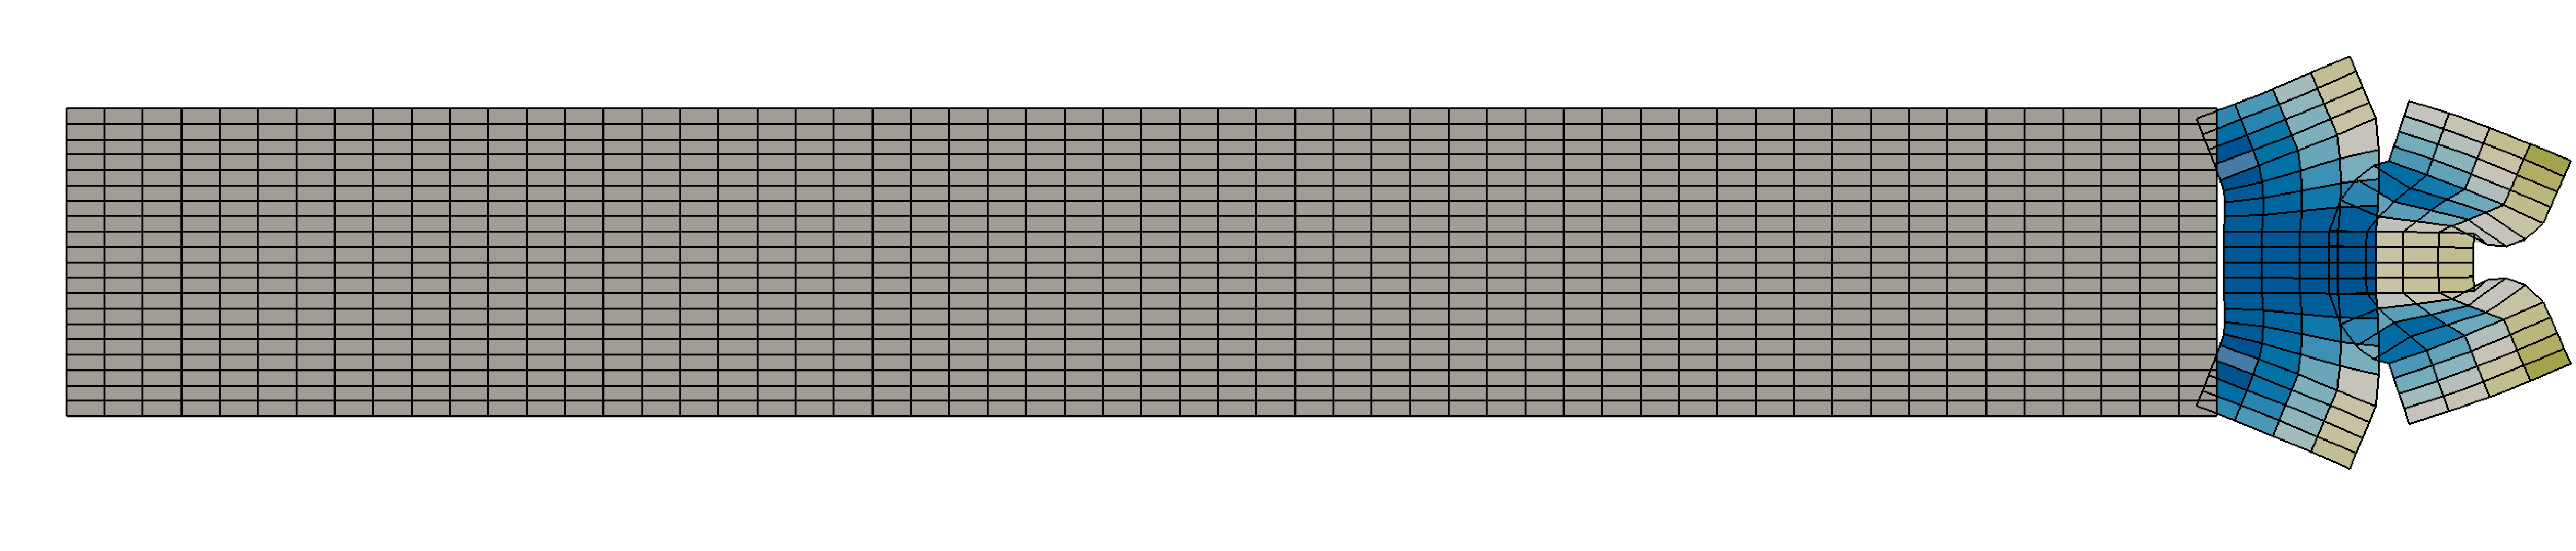
\includegraphics[width=0.9\linewidth, height=5cm]{/home/lukas/Desktop/SA_Thesis/studies/2016-08-18_EigenvalueDistribution/setup/feti1_iter1.png} 

\begin{tikzpicture}
\def\ydist{-5.5}
\node[inner sep=0pt] (russell) at (0,0)
    {\includegraphics[width=.5\textwidth]{\studypath/2016-08-10_Partitioning/setup/regular_6x6.png}};
\node at (0,0.45*\ydist) [anchor=east, scale=1] {\contour{white}{iteration 1}};


\node[inner sep=0pt] (russell) at (.5\textwidth,0)
    {\includegraphics[width=.5\textwidth]{\studypath/2016-08-10_Partitioning/setup/chaco_6x6.png}};
\node at (.5\textwidth,0.45*\ydist) [anchor=east, scale=1] {\contour{white}{iteration 2}};




\node[inner sep=0pt] (russell) at (0,\ydist)
    {\includegraphics[width=.5\textwidth]{\studypath/2016-08-10_Partitioning/setup/chaco_11x1.png}};
\node at (0,\ydist+0.45*\ydist) [anchor=east, scale=1] {\contour{white}{iteration 5}};

\node[inner sep=0pt] (russell) at (.5\textwidth,\ydist)
    {\includegraphics[width=.5\textwidth]{\studypath/2016-08-10_Partitioning/setup/chaco_1x11.png}};
\node at (.5\textwidth,\ydist+0.45*\ydist) [anchor=east, scale=1] {\contour{white}{iteration 8}};


\end{tikzpicture}








\begin{figure}[htbp]
    \centering
    \begin{subfigure}[b]{0.3\textwidth}
        \includegraphics[width=\textwidth]{/home/lukas/Desktop/SA_Thesis/studies/2016-08-10_Partitioning/setup/regular_6x6.png}
        \caption{Testing of the X-axis.}
        \label{rfidtest_xaxis}
    \end{subfigure}
    \begin{subfigure}[b]{0.3\textwidth}
        \includegraphics[width=\textwidth]{/home/lukas/Desktop/SA_Thesis/studies/2016-08-10_Partitioning/setup/regular_6x6.png}
        \caption{Testing of the Y-axis.}
        \label{rfidtest_yaxis}
    \end{subfigure}
    \begin{subfigure}[b]{0.3\textwidth}
        \includegraphics[width=\textwidth]{/home/lukas/Desktop/SA_Thesis/studies/2016-08-10_Partitioning/setup/regular_6x6.png}
        \caption{Testing of the Z-axis.}
        \label{rfidtest_zaxis}
    \end{subfigure}
    \caption[RFID tag read-range testing]{RFID tag read-range testing setup. In all tests, the finger moves towards along an axis towards the tag.}
    \label{rfidtag_testing}
\end{figure}







%\begin{tikzpicture}
% \begin{groupplot}[
%group style = {group size = 2 by 2, horizontal sep=2.0cm, vertical sep=1.5cm},
%height = 5cm,
%width = 5cm,
%]
%
%
%\nextgroupplot
%\node[inner sep=0pt] (russell) at (0,0)
%    {\includegraphics[width=.5\textwidth]{\studypath/2016-08-10_Partitioning/setup/regular_6x6.png}};
%\node at (0,0.45*\ydist) [anchor=east, scale=1] {\contour{white}{iteration 1}};
%
%\nextgroupplot
%\node[inner sep=0pt] (russell) at (0,0)
%    {\includegraphics[width=.5\textwidth]{\studypath/2016-08-10_Partitioning/setup/regular_6x6.png}};
%\node at (0,0.45*\ydist) [anchor=east, scale=1] {\contour{white}{iteration 1}};
%
%\nextgroupplot
%\node[inner sep=0pt] (russell) at (0,0)
%    {\includegraphics[width=.5\textwidth]{\studypath/2016-08-10_Partitioning/setup/regular_6x6.png}};
%\node at (0,0.45*\ydist) [anchor=east, scale=1] {\contour{white}{iteration 1}};
%
%\nextgroupplot
%\node[inner sep=0pt] (russell) at (0,0)
%    {\includegraphics[width=.5\textwidth]{\studypath/2016-08-10_Partitioning/setup/regular_6x6.png}};
%\node at (0,0.45*\ydist) [anchor=east, scale=1] {\contour{white}{iteration 1}};
%
%
%\end{groupplot}
%\end{tikzpicture}


\end{document}